\section{Procedimiento Laboratorio} \pagenumbering{roman}
\subsection{Imanes}

\subsubsection{Determine las líneas de campo de los diferentes imanes}
Con las limaduras de hierro determine las líneas de campo de los diferentes
imanes, como se muestra en la figura adjunta.


\subsubsection{Encontrar los polos norte y sur}
Con dos imanes encontrar los polos norte y sur de cada uno de ellos.


\subsubsection{Para dos imanes comprobar}
Para dos imanes comprobar que polos magnéticos del mismo tipo se repelen y polos
magnéticos de distinto tipo se atraen.

Se trata de manejar una pareja de imanes y observar las posiciones en donde la
atracción es máxima y las posiciones en donde la repulsión es máxima.
Igualmente, se trata de visualizar el campo magnético con limaduras de hierro en
las siguientes situaciones:

\begin{itemize}
    \item Un imán.
    \item Dos imanes con polos idénticos enfrentados.
    \item Dos imanes con polos opuestos enfrentados.
\end{itemize}


\subsubsection{Teslámetro}
Con ayuda del teslámetro mida el campo magnético para una distancia constante en
diferentes imanes y determine cual tiene mayor fuerza magnética.


\subsubsection{Geometría del teslámetro}
De acuerdo con la geometría del teslámetro construya la siguiente tabla,
midiendo el campo magnético de tres imanes diferentes a diferentes distancias.


\begin{figure}[H]
    \centering
    \begin{subfigure}[b]{0.8\textwidth}
        \centering
        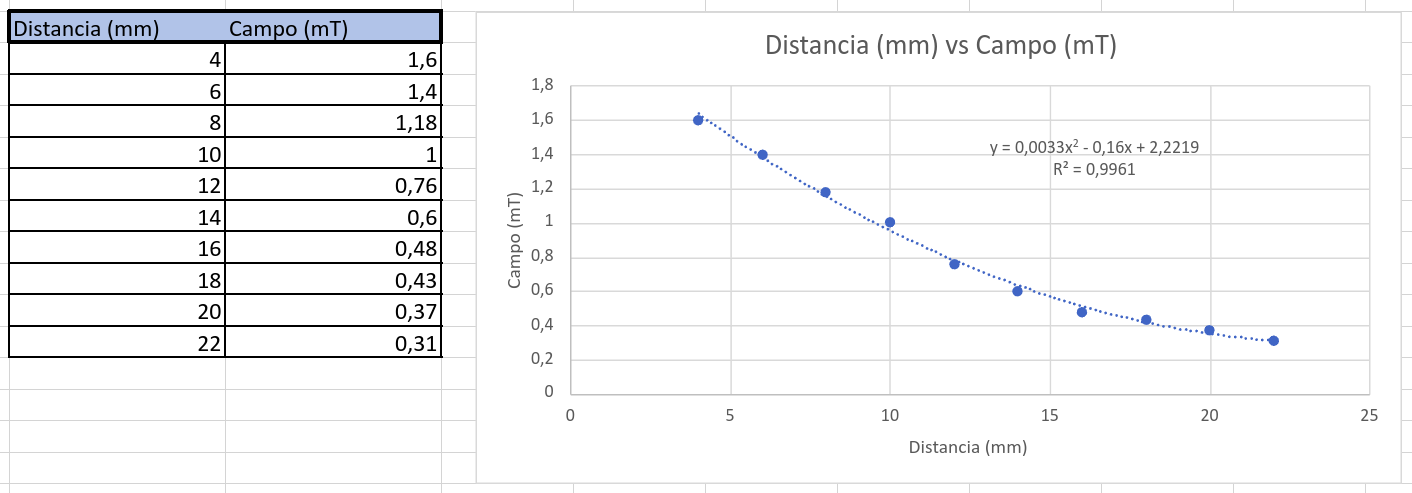
\includegraphics[width=\textwidth]{Figures/0. General/1.5.png}
        \caption{\textit{B vs d}}
        \label{fig: style 1 B vs d}
    \end{subfigure}
\end{figure}


\subsubsection{¿Cómo varía \textit{B} con \textit{d}?}
Analizando los resultados de la tabla y el grafico \textit{B vs d} que estos
resultados nos brindan, se comprueba que la medida del campo magnético depende
indirectamente de la distancia a la cual este se está midiendo, dado que este se
hace menor a medida que aumenta la distancia, y aumenta al reducir la distancia
del imán que lo genera con el teslámetro que lo mide.


\subsubsection{¿Qué significado tiene la expresión de que un imán es muy potente?}
Esta expresión hace referencia a su densidad de líneas de campo magnético,
porque al ser mayor, la fuerza magnética con la que atrae a otros imanes, o
algunos materiales metalicosmetálicos será mayor.


\subsubsection{Comparado con el campo magnético de la Tierra}
Comparado con el campo magnético de la Tierra, ¿qué orden de magnitud tienen los
valores que usted midió para el campo magnético de los imanes?\\

La tierra funciona como un gran imán cuya magnitud oscila entre:\\

\(2.5\times10^{-5}\) y \(6.5\times10^{-5}\) (T) Teslas siendo mayor en los polos
y menor cerca de la line del ecuador. Para la respuesta tendremos en cuenta que
la magnitud del campo magnético de la tierra medido en la superficie de la
tierra puede alcanzar un valor máximo de \(6.5\times10^{-5}\) (T) y que el
valor de campo magnético más grande alcanzado por uno de los imanes en el
laboratorio fue de \(4.02\times10^{-2}\).\\

Al analizar esto, se puede observar que el campo magnético de los imanes tiene
un orden de \(10^{-2}\) el cual es mil veces mayor ok que el de la tierra
que tiene un orden de magnitud de \(10^{-5}\).


\subsection{Campo magnético terrestre}

\subsubsection{Montaje Figura 2}
Realice el montaje mostrado en la Figura 2.


\subsubsection{brújula en el centro}
Sin haber encendido la fuente, coloque la brújula en el centro de las bobinas.
La dirección hacia donde apunta la brújula, es la dirección del campo magnético
terrestre. Ubique las bobinas de modo que su plano esté en la dirección delcampo
magnético terrestre, o sea que su eje este en la dirección este-oeste, como se
observa en la Figura 2.


\subsubsection{Encontrar los polos norte y sur}
Encienda la fuente de voltaje y ajuste una corriente hasta que la aguja de la
brújula se ubique en \(\phi = 10^\circ\). La aguja de la brújula se orienta en dirección del campo
magnético resultante de combinar el campo magnético de las bobinas y el campo
magnético terrestre. Tome la dirección norte-sur para medir los ángulos, es
decir, tome como la orientación de la aguja de la brújula cuando la corriente
por las bobinas es cero, como se observa en la Figura 2. Registre la medida de
la corriente mostrada en el miliamperímetro, en la casilla de la tabla que
aparece a continuación y calcule \textit{BH} con la relación (6): Sí no es posible colocar
la aguja de la brújula en los ángulos sugeridos, defina usted por lo menos 7
posiciones angulares y realice:


\begin{figure}[H]
    \centering
    \begin{subfigure}[b]{\textwidth}
        \centering
        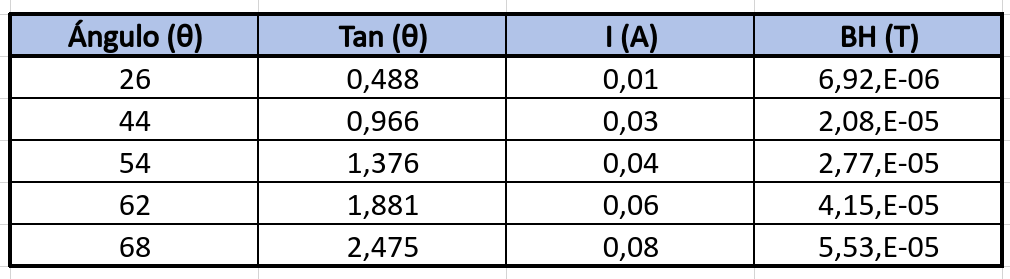
\includegraphics[width=\textwidth]{Figures/0. General/2.3.1.png}
        \caption{\textit{Tabla 1.2.3.1}}
    \end{subfigure}
\end{figure}

\begin{figure}[H]
    \centering
    \begin{subfigure}[b]{0.6\textwidth}
        \centering
        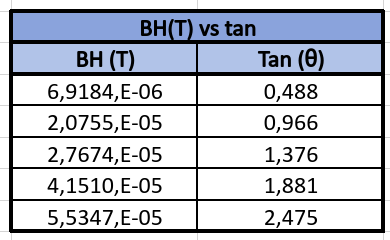
\includegraphics[width=\textwidth]{Figures/0. General/2.3.2.png}
        \caption{\textit{Tabla 1.2.3.2}}
    \end{subfigure}
\end{figure}



\subsubsection{Grafique \textit{BH(I)} vs \textit{tan\((\phi)\)}}
Grafique \textit{BH(I)} vs \textit{tan\((\phi)\)}:

\begin{figure}[H]
    \centering
    \begin{subfigure}[b]{\textwidth}
        \centering
        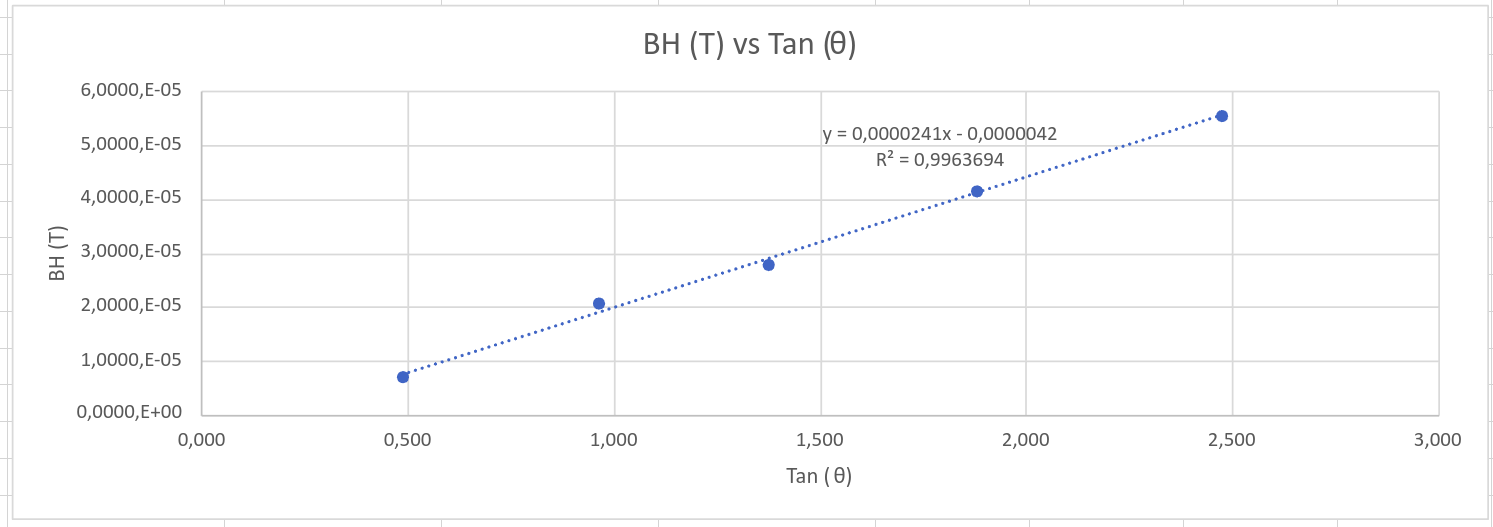
\includegraphics[width=\textwidth]{Figures/0. General/2.4.png}
        \caption{\textit{BH(I)} vs \textit{tan\((\phi)\)}}
    \end{subfigure}
\end{figure}


\subsubsection{campo magnético terrestre}
Encuentre el campo magnético terrestre haciendo uso de la pendiente de la
gráfica anterior (use regresión lineal).\\

Teniendo en cuenta la fórmula de la recta:
\[ y = mx\]

Y teniendo en cuenta la ecuación 7 de la orientación del ángulo de la brújula
sometida a ambos campos:

\[ Tan_{(\phi)} = \frac{B_{H}(I)}{B_{T}} \]

Despejemos $B_{H}$

\[ B_{H}(I) = Tan_{(\phi)} \times B_{T} \]

Ahora relacionamos que en el eje coordenado y tenemos $B_{H}(I)$ (campo
magnético de las bobinas) y en el eje coordenado x tenemos $Tan_{(\phi)}$ (el
ángulo resultante de la acción de los dos campos magnéticos sobre la brújula)
podemos decir que $m = B_{T}$, es decir $B_{T}$ es la pendiente, entonces la
pendiente de la gráfica realizada debe ser igual o muy parecida al campo
mágnetico de la tierra.


\subsubsection{Porcentaje de error relativo}
Para evaluar el porcentaje de error relativo, del campo magnético terrestre
hallado experimentalmente, consulte en la red (en una fuente de información
confiable) el valor del campo magnético en la ciudad de Medellín.\\

El valor del campo magnético en la ciudad de Medellín es de:

\[ 3.11861\times10^{-5} T (Teslas)\]

Entonces el errror relativo es igual a:

\[ \%Error relativo = \frac{|3.11861\times10^{-5} - 2.41\times10^{-5}|}{3.11861\times10^{-5}}\]

\[ \%Error relativo = 22.72\%\]


\subsubsection{Qué factores pueden afectar el cálculo experimental?}
¿Qué factores pueden afectar el cálculo experimental del campo magnético
terrestre en el laboratorio?

Es posible que al medir la dirección de la brújula se vea afectada por otros
objetos que generen campo magnético más cercano que lo que esta la brújula a los
polos, por ejemplo, un imán o también ciertos movimientos involuntarios que se
le hagan al soporte de la brújula.


\subsubsection{Conclusiones}
En este informe número 5, pudimos ver el comportamiento magnético con
experimentos prácticos para observar el campo magnético con la limadura de
hierro, la interacción entre polos (norte y sur), además, experimentando más a fondo
logramos ver con diferentes imanes su campo dependiendo de su distancia y como
este es proporcional a esta, también con esto logramos observar el campo
magnético terrestre con un 22.72\% de margen de error que se pudo ver afectado por
diversos factores como otro campo magnético más cercano a la brújula, tal vez
pequeños movimientos involuntarios en el dispositivo, o cabe la posibilidad que
la precisión de fabricación de la brújula no sea completamente precisa.
